% Background section
\subsection{Phase Transitions and Emergence in Complex Systems}

\subsubsection{Phase Transitions}

Phase transitions traditionally refer to qualitative changes in the state of a physical system, such as the transition from liquid to gas or the onset of magnetization in ferromagnets. The hallmark of these transitions is a sudden change in system properties at a critical point, characterized by power-law scaling behaviors and critical exponents \citep{newman2003structure, bak1987self, stanley1971phase}. In complex systems, phase transitions extend beyond physical phenomena to include abrupt shifts in collective behavior across diverse domains \citep{watts2002simple, scheffer2009critical}. Phase transitions in complex systems typically involve the emergence of new patterns or structures at a system level that are not present in individual components \citep{anderson1972more}. They are studied using a variety of mathematical and computational tools, including network theory, statistical physics, and dynamical systems theory \citep{barabasi1999emergence, strogatz2001exploring} and can be quantified through observables such as order parameters, susceptibility, and correlation functions \citep{stanley1999scaling, goldenfeld1992lectures}.

\subsubsection{Emergence}

Emergence in complex systems refers to the appearance of novel properties or behaviors at higher levels of organization that are not present at lower levels \citep{holland1998emergence, anderson1972more}. Emergent phenomena often arise from the interactions and collective dynamics of individual components, leading to the formation of new structures, patterns, or functions \citep{kauffman1993origins, gell1994quark}. Examples of emergence include the self-organization of biological systems, the emergence of intelligence in social networks, and the formation of traffic patterns in urban systems \citep{camazine2003self, haken1983synergetics}.

Phase transitions can be viewed as a subset of emergent phenomena, where the abrupt changes in system behavior correspond to the emergence of new collective states \citep{sethna2006statistical, goldenfeld1992lectures}. All phase transitions involve emergence, but not all emergent phenomena are phase transitions \citep{bar2013computability}.

\subsection{Modeling Phase Transitions and Emergence}

\subsubsection{Physical Models}

In physics, phase transitions are often modeled using statistical mechanics, where the system's behavior is described in terms of energy, entropy, and temperature \citep{stanley1971phase, kadanoff2000statistical}. The Ising model, Potts model, and percolation theory are classic examples of physical models used to study phase transitions \citep{onsager1944crystal, stauffer2018introduction}. These models capture the interactions between individual components and the emergence of collective behavior at critical points \citep{binney1992theory}. They, however, have limitations in capturing the complexity of real-world systems, such as biological, social, and technological networks but tend to be more mathematically tractable for detailed analysis \citep{newman2011structure}.

\subsubsection{Network Models}

Networks have been used since the early 20th century to model complex systems, representing entities as nodes and interactions as edges \citep{watts1998collective, barabasi1999emergence}. Formally, a network is represented as a graph $G = (V, E)$ where $V$ is a set of vertices (nodes) and $E \subseteq V \times V$ is a set of edges (links). For directed networks, edges are ordered pairs $(u, v) \in E$ indicating a directed relationship from node $u$ to node $v$. For undirected networks, edges are unordered pairs $\{u, v\} \in E$.

The structure of a network can be represented by its adjacency matrix $A$, where:
\begin{equation}
A_{ij} =
\begin{cases}
1 & \text{if } (i,j) \in E \text{ (or } \{i,j\} \in E \text{ for undirected graphs)} \\
0 & \text{otherwise}
\end{cases}
\end{equation}

\begin{figure}[htbp]
    \centering
    \includegraphics[width=\textwidth]{figures/network_models-1.png}
    \caption{Network models and emergent phenomena. Top left: An undirected network with community structure. Top right: A directed weighted ne
    twork with hub-and-spoke architecture showing asymmetric relationships. Bottom: Emergent    phenomena including phase transitions (formatio
    n of a giant connected component when edge probability exceeds critical threshold $p_c$)    cascading processes (diffusion and contagion spread
    ing through a network).}
    \label{fig:network_models}
\end{figure}

For weighted networks, $A_{ij}$ represents the strength of the connection between nodes $i$ and $j$. Several key metrics characterize network properties:

\begin{itemize}
    \item \textbf{Degree distribution} $P(k)$: The probability that a randomly selected node has $k$ connections
    \item \textbf{Clustering coefficient} $C_i$: For a node $i$ with $k_i$ neighbors, $C_i = \frac{2e_i}{k_i(k_i-1)}$ where $e_i$ is the number of links between the neighbors
    \item \textbf{Path length} $d(i,j)$: The minimum number of edges traversed to reach node $j$ from node $i$
    \item \textbf{Betweenness centrality} $B(v)$: $B(v) = \sum_{s \neq v \neq t} \frac{\sigma_{st}(v)}{\sigma_{st}}$ where $\sigma_{st}$ is the number of shortest paths from $s$ to $t$ and $\sigma_{st}(v)$ is the number of those paths passing through $v$
\end{itemize}

Critical phenomena in networks, such as phase transitions, often manifest through sudden changes in global network properties. For instance, the emergence of a giant connected component in random networks occurs at a critical probability $p_c = \frac{1}{N}$, where $N$ is the number of nodes \citep{erdos1960evolution}.

Network models have been successful in capturing the structure and dynamics of a wide range of systems, including social networks, biological networks, and technological networks \citep{newman2003structure, albert2002statistical, strogatz2001exploring}. Networks are both a mathematically rigorous framework as well as intuitive and visually appealing, making them a popular choice for modeling complex systems \citep{newman2010networks}. Networks can capture the emergence of collective behavior through the study of network motifs, community structure, and dynamical processes on networks \citep{milo2002network, fortunato2010community, barrat2008dynamical}, and has attracted significant attention in recent years \citep{barabasi2016network}.

\subsubsection{From Networks to Simplicial Complexes}

Simplicial complexes generalize networks by incorporating higher-order interactions. Simplicial complexes can be thought of as triangles of various dimensions - vertices (0-simplices), edges (1-simplices), triangles (2-simplices), tetrahedra (3-simplices), and so on \citep{petri2014homological} connected together either via shared vertices, edges, or faces.

Formally, a simplicial complex $K$ on a vertex set $V$ is a collection of subsets of $V$ (called simplices) such that:
\begin{itemize}
    \item For every vertex $v \in V$, $\{v\} \in K$ (0-simplex)
    \item If $\sigma \in K$ and $\tau \subset \sigma$, then $\tau \in K$ (closure property)
\end{itemize}

A $k$-simplex $\sigma = [v_0, v_1, ..., v_k]$ represents an interaction between $k+1$ vertices. For example:
\begin{itemize}
    \item A 0-simplex is a vertex
    \item A 1-simplex is an edge (pairwise interaction)
    \item A 2-simplex is a filled triangle (three-way interaction)
    \item A 3-simplex is a solid tetrahedron (four-way interaction)
    \item and so on
\end{itemize}

\begin{figure}[htbp]
    \centering
    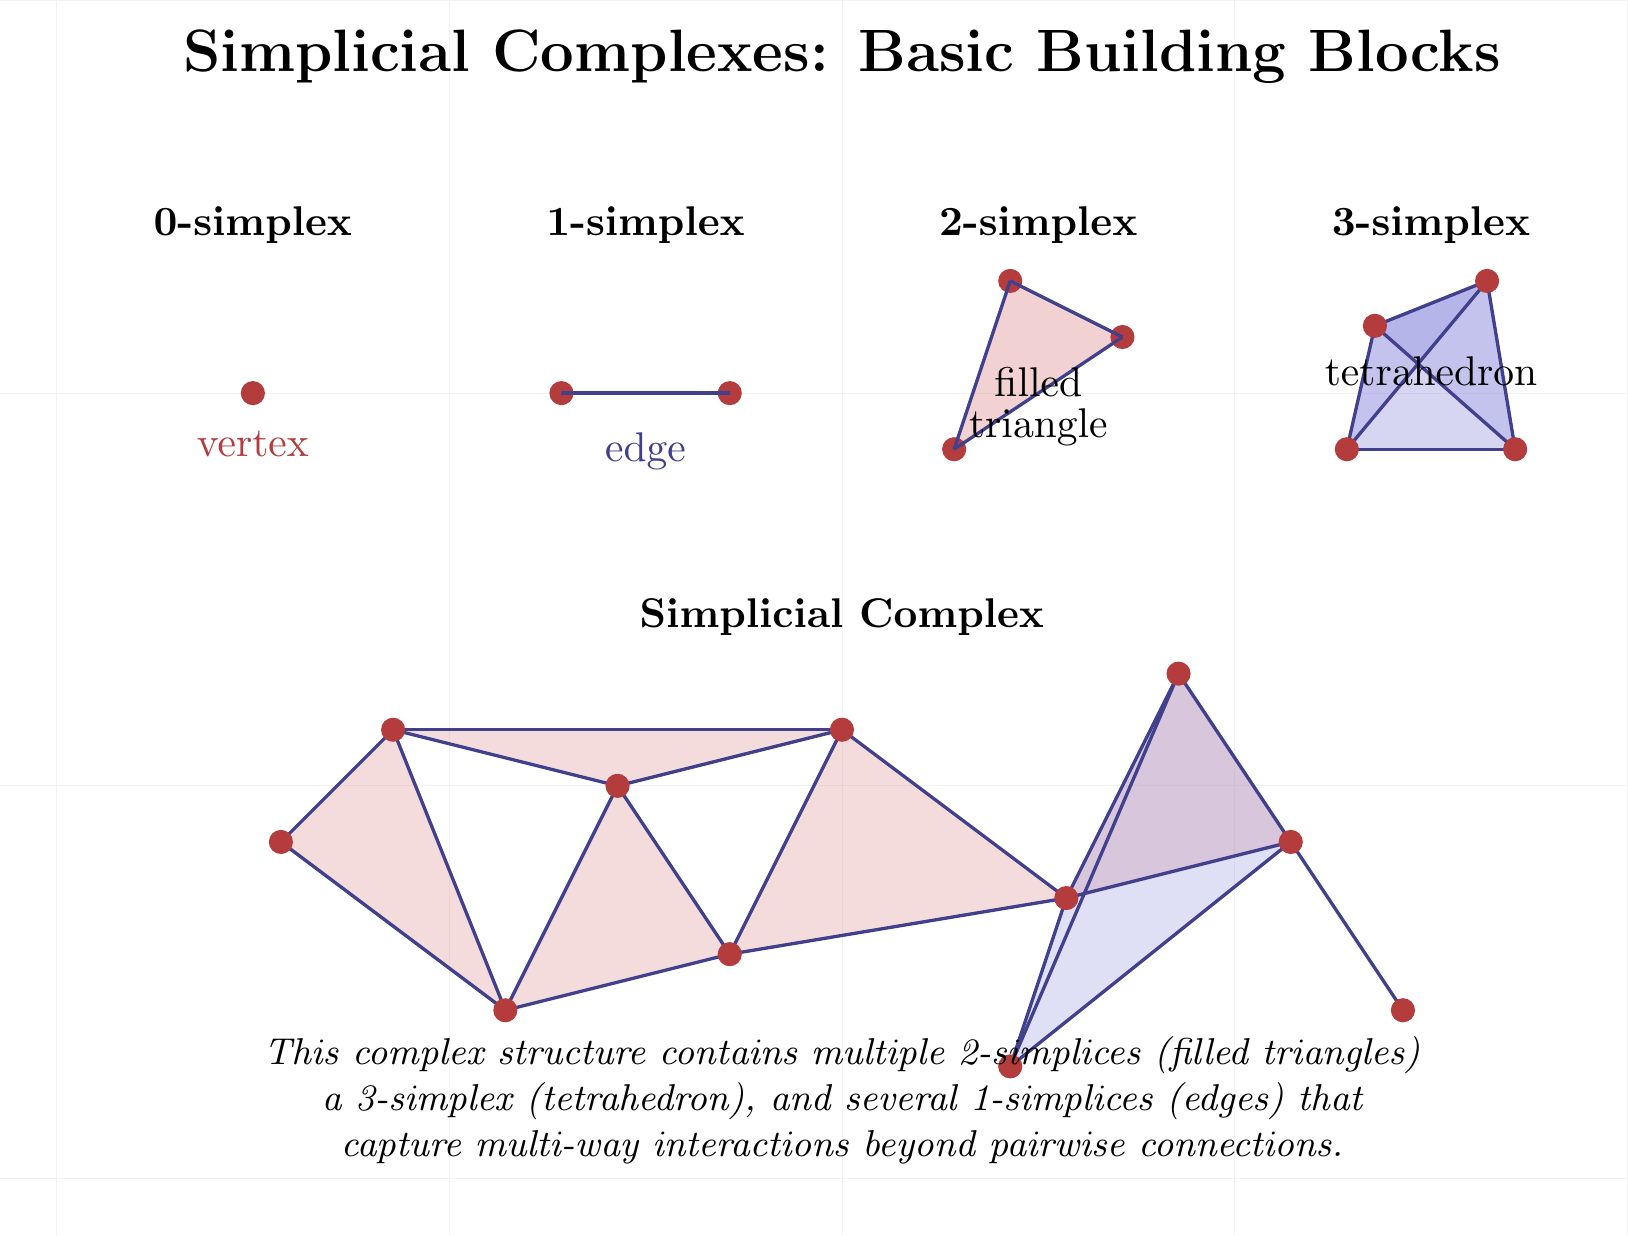
\includegraphics[width=\textwidth]{figures/simplicial_complexes-1.png}
    \caption{Visual representation of simplicial complexes. The top row shows individual simplices of different dimensions (0-simplex, 1-simplex, 2-simplex, and 3-simplex). The bottom part shows a more complex simplicial complex with multiple 2-simplices (filled triangles), a 3-simplex (tetrahedron), and connecting 1-simplices (edges) that capture multi-way interactions beyond pairwise connections.}
    \label{fig:simplicial_complexes}
\end{figure}

Several researchers have successfully applied simplicial complexes to model complex systems. \citet{petri2014homological} used simplicial complexes to analyze brain functional networks, revealing topological structures that correlate with cognitive states. \citet{giusti2016two} demonstrated how simplicial complexes can capture neural coding schemes beyond what traditional network models could represent. \citet{sizemore2018importance} showed how clique topology in neural systems provides insights into brain development and function.

While simplicial complexes offer significant advantages over traditional networks, they have inherent limitations:
\begin{itemize}
    \item They are \textit{undirected}, with no natural way to represent asymmetric interactions
    \item \textit{Temporal dynamics} are challenging to model in simplicial complexes
\end{itemize}

\subsection{Opetopes}

Originally developed in higher category theory \citep{cheng2004higher, kock2010polynomial}, opetopes are higher-dimensional shapes defined recursively by their boundaries, which are themselves opetopes of lower dimensions. Dimensions here refer to the number of vertices in the opetope, with a 0-dimensional opetope being a point, a 1-dimensional opetope being a directed edge, and so on. Opetopes of higher dimensions are constructed from lower-dimensional opetopes by gluing them together along their boundaries. To further simply using an example, an opetope can be a 2D square going along clockwise, thus not only capturing the shape but also the directionality of the shape.

\begin{figure}[htbp]
    \centering
    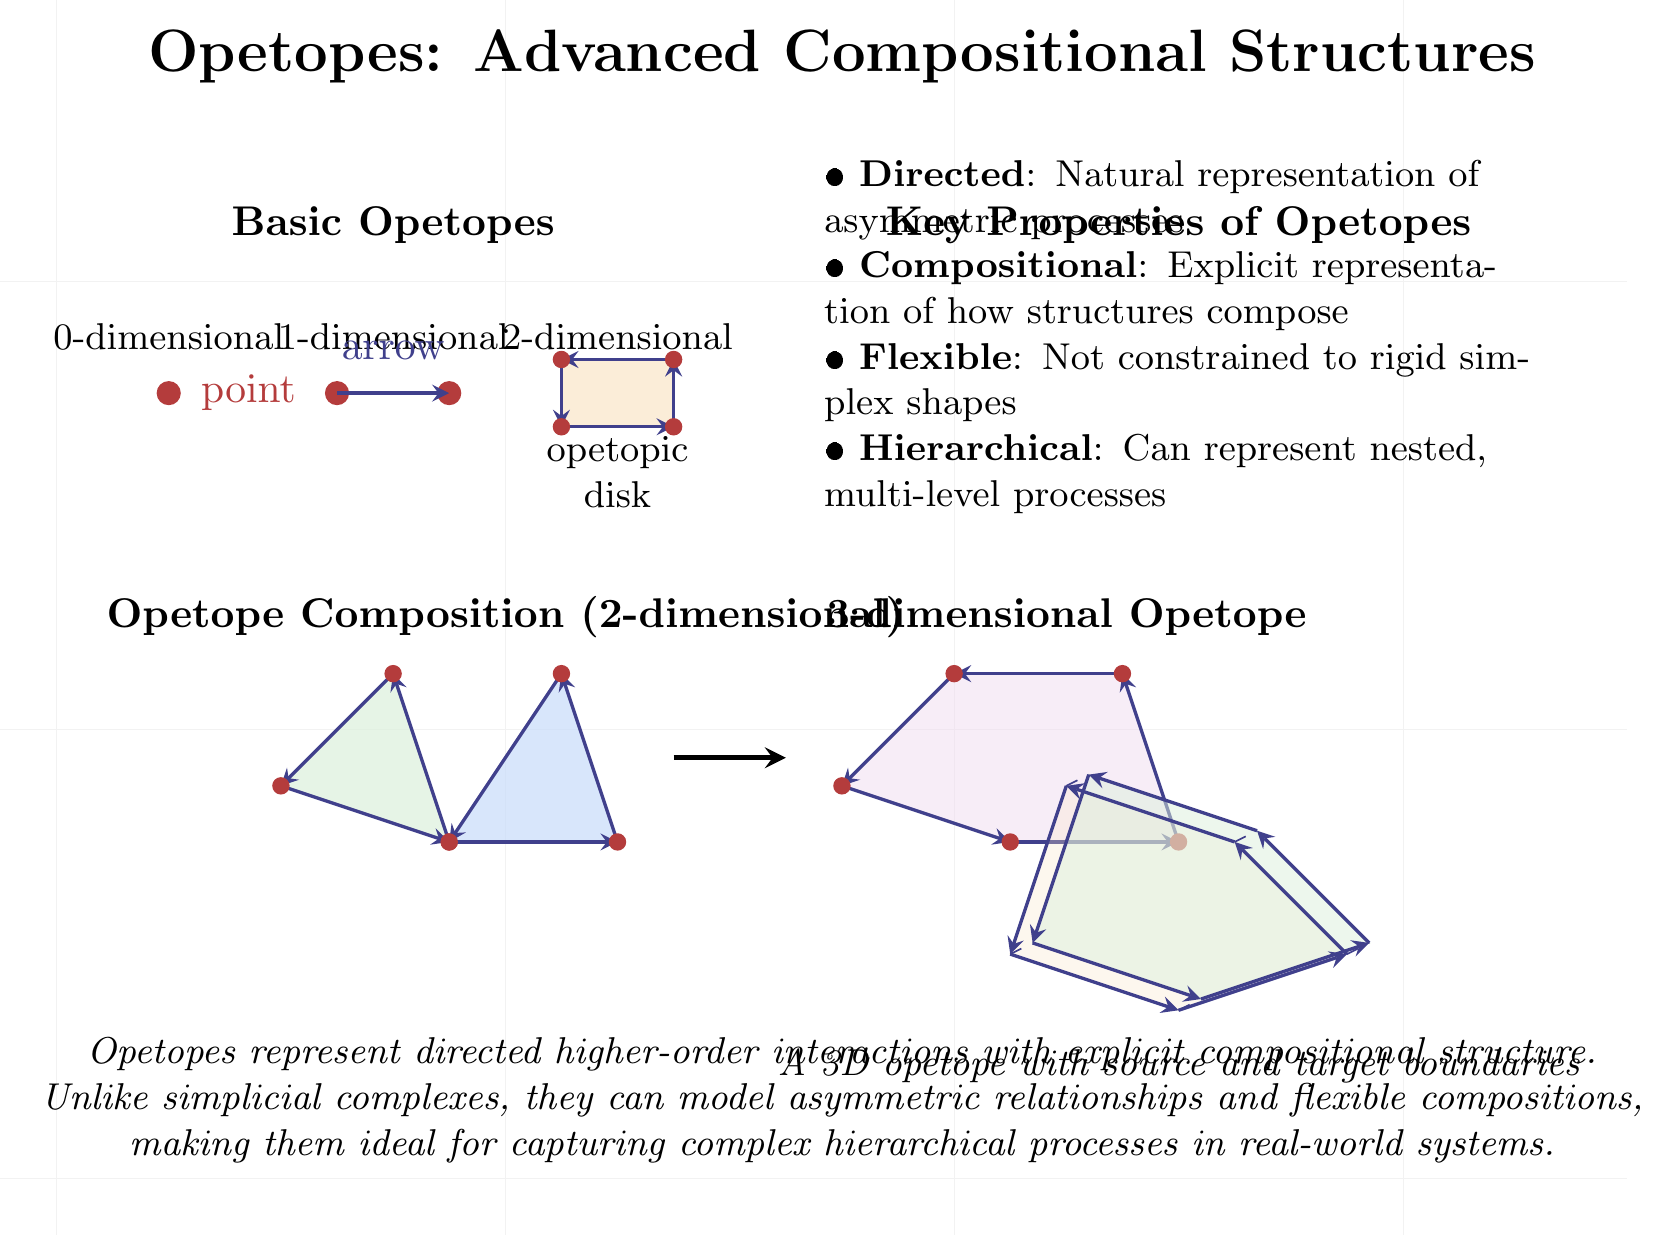
\includegraphics[width=\textwidth]{figures/opetope_structures-1.png}
    \caption{Visual representation of opetopes and their properties. Top: Basic opetopes of different dimensions from 0D to 2D, along with key properties that distinguish them from simplicial complexes.}
    \label{fig:opetope_structures}
\end{figure}

\subsubsection{Formal Definition}

Formally, an $n$-dimensional opetope can be defined as:

\begin{itemize}
    \item A 0-dimensional opetope is a point
    \item A 1-dimensional opetope is a directed arrow between points
    \item For $n>1$, an $n$-dimensional opetope has:
    \begin{itemize}
        \item A source boundary, consisting of $(n-1)$-dimensional opetopes arranged in a tree-like pattern
        \item A target boundary, consisting of a single $(n-1)$-dimensional opetope
    \end{itemize}
\end{itemize}

The mathematical framework of opetopes is closely related to operads, higher categories, and polynomial functors \citep{baez2020network, leinster2004higher}. These connections provide rich analytical tools for understanding opetopic models.

Opetopes can be formalized in dependent type theory \citep{finster2019opetopic}, providing a foundation for mechanical verification of opetopic models. This connection bridges opetopic modeling with formal logic and programming language theory. In this work, we use Lean the theorem prover to model opetopes and show how to use them to construct complex systems models.
